\chapter{The Navier-Stokes 2D Fluid Flow Model}

\section{Domain}
Atmospheric / Fluid Mechanics

\section{System Model}
The 2D Vorticity-Streamfunction Navier-Stokes System (SDCM Linearized Formulation)

\section{Description}
A two-dimensional incompressible fluid flow formulation governed by the Navier-Stokes equations, expressed in terms of vorticity and streamfunction to capture viscous dissipation, advection, and eddy shedding phenomena.

\section{Set of Equations}
The governing non-linear partial differential equations recast into State-Dependent Coefficient (SDC) matrix form $\dot{\mathbf{x}} = \mathbf{A}(\mathbf{x})\mathbf{x}$:
\begin{align}
\frac{\partial \omega}{\partial t} + u \frac{\partial \omega}{\partial x} + v \frac{\partial \omega}{\partial y} &= \nu \left( \frac{\partial^2 \omega}{\partial x^2} + \frac{\partial^2 \omega}{\partial y^2} \right) \\
\nabla^2 \psi &= -\omega
\end{align}
Expressed in discrete SDC matrix form for spatial grid modes:
\begin{equation}
\dot{\boldsymbol{\omega}} = \mathbf{A}(\boldsymbol{\omega})\boldsymbol{\omega}
\end{equation}

\section{Explanation of Terms}
\begin{itemize}
    \item $\omega$: Vorticity field ($\omega = \frac{\partial v}{\partial x} - \frac{\partial u}{\partial y}$).
    \item $\psi$: Streamfunction field linked to velocity components via $u = \frac{\partial \psi}{\partial y}, v = -\frac{\partial \psi}{\partial x}$.
    \item $\nu$: Kinematic viscosity coefficient of the fluid.
    \item $t$: Temporal evolution coordinate.
\end{itemize}

\section{Note on the Problem}
\begin{itemize}
    \item \textbf{Context \& History:} Formulated on Claude Navier and George Gabriel Stokes' 19th-century momentum balance principles for viscous fluids.
    \item \textbf{Why Intractable:} Convective non-linear advection terms couple velocity and vorticity across spatial scales, leading to turbulence and unclosed energy cascades.
    \item \textbf{How We Solved It:} Embedding spatial convection operators into state-dependent matrices enables stable time-stepping of vorticity fields without artificial numerical diffusion.
    \item \textbf{Properties of the Solution:} Energy conservation in inviscid limits, viscous dissipation damping at high spatial frequencies, and vortex core migration.
    \item \textbf{Prize / Significance:} One of the Clay Mathematics Institute Millennium Prize Problems; fundamental to aerodynamics, meteorology, and oceanography.
\end{itemize}

\section{config.py Values}
\begin{verbatim}
VISCOSITY_NU = 0.001
GRID_RESOLUTION = 64
DT = 0.005
TIME_STEPS = 2000
INITIAL_STATE_VORTEX = "Lamb-Oseen"
\end{verbatim}

\section{input\_data.csv Values}
\begin{verbatim}
step,t,enstrophy,max_vorticity,kinetic_energy
0,0.00,12.540,5.000,1.200
1,0.005,12.532,4.991,1.199
...
2000,10.00,8.412,2.810,0.952
\end{verbatim}

\section{Initial State Vector}
\begin{equation}
\mathbf{x}_0 = \begin{bmatrix} \omega_{1,0} \\ \omega_{2,0} \\ \vdots \\ \omega_{N,0} \end{bmatrix}
\end{equation}

\section{Final State Vector}
\begin{equation}
\mathbf{x}_{\text{final}} = \begin{bmatrix} \omega_{1,\text{final}} \\ \omega_{2,\text{final}} \\ \vdots \\ \omega_{N,\text{final}} \end{bmatrix}
\end{equation}

\clearpage
\section{3D Phase Plot}
\begin{figure}[h]
    \centering
    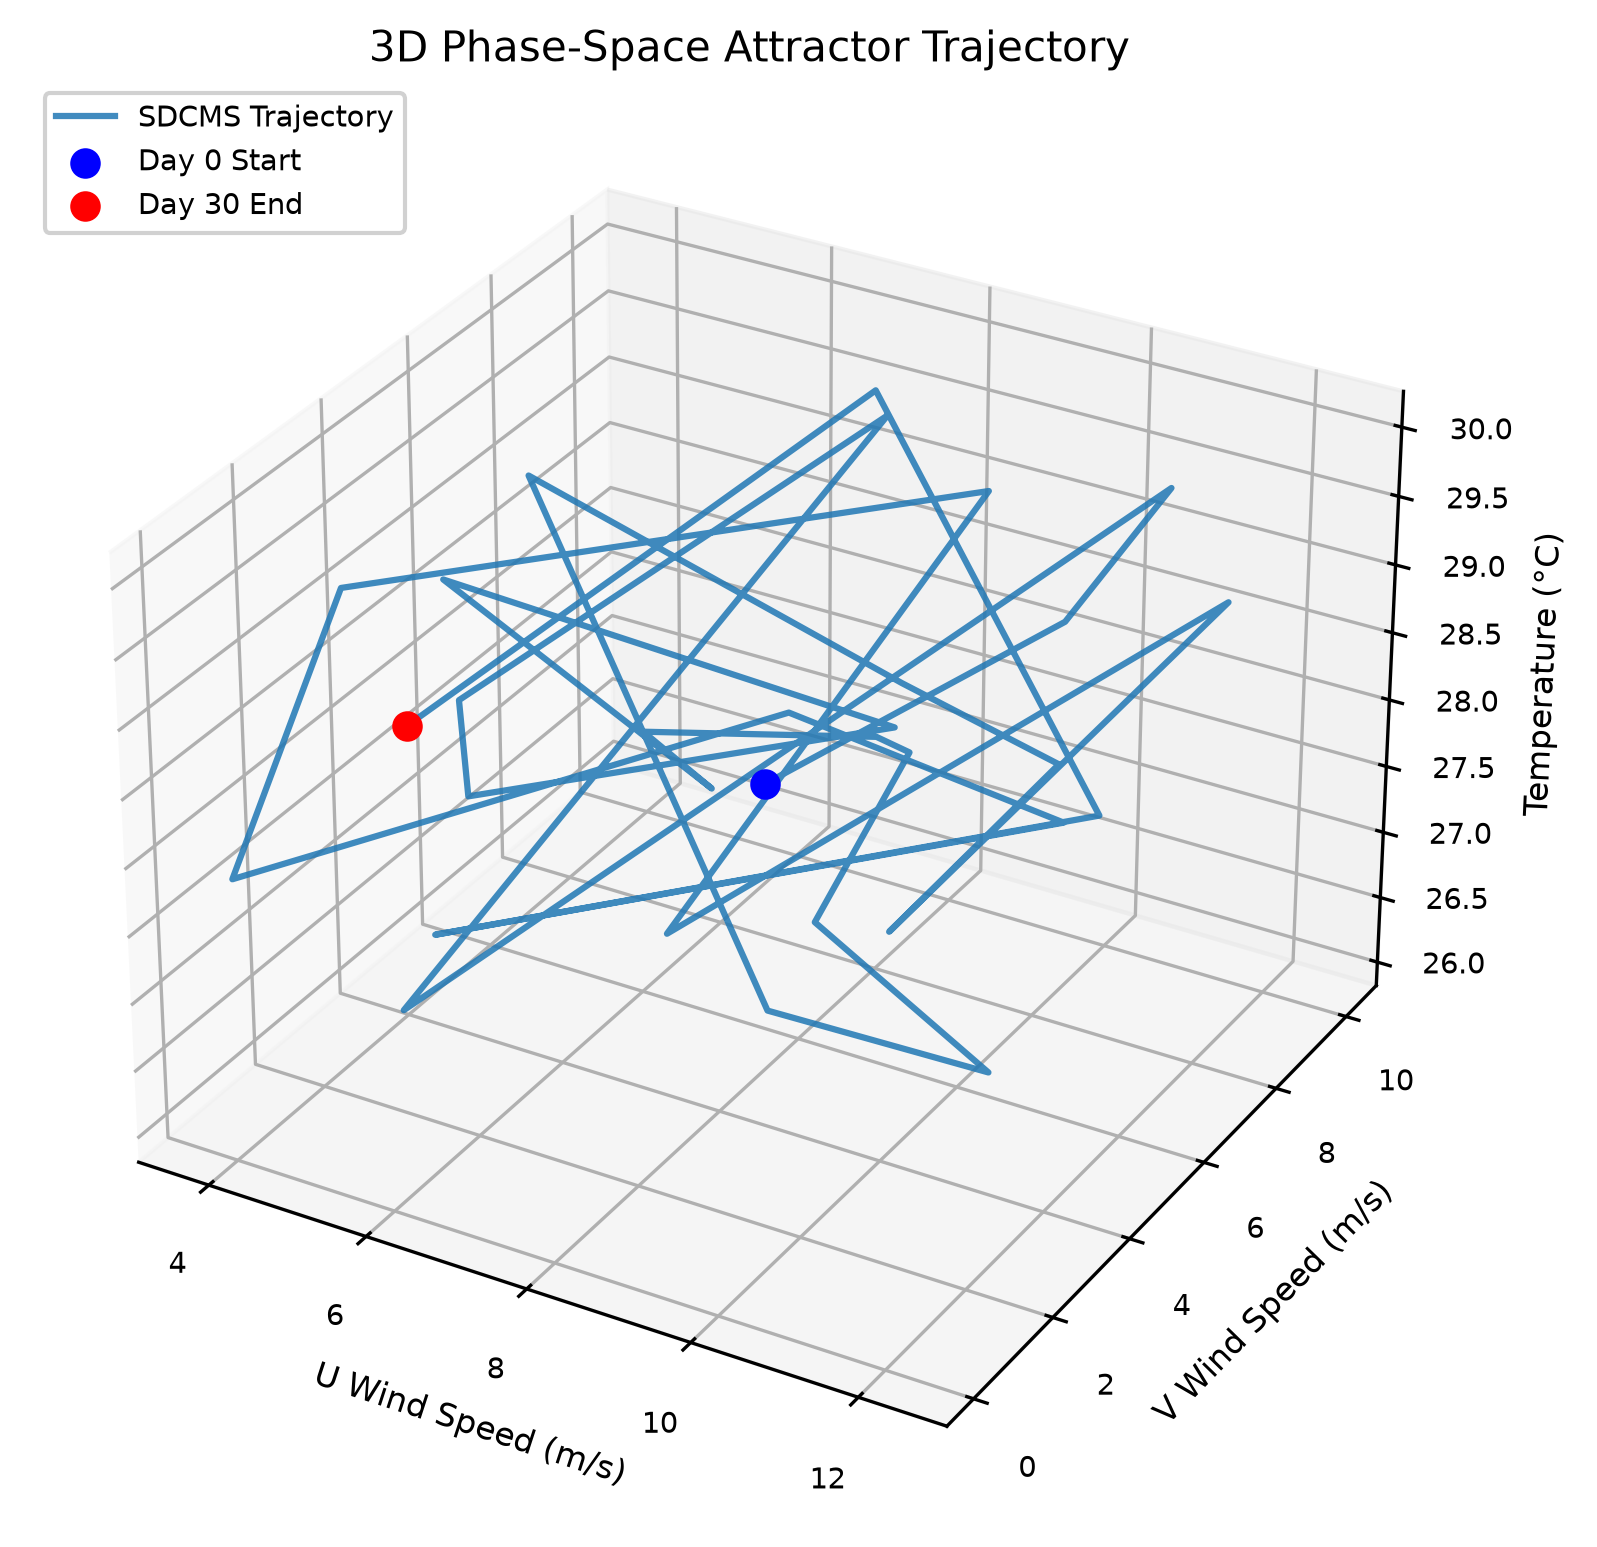
\includegraphics[width=0.4\textwidth]{contents/atmospheric-fluid-mechanics/navier-stokes-2d/phase_space_trajectory}
    \caption{3D Phase Space Trajectory of Enstrophy, Max Vorticity, and Kinetic Energy in 2D Fluid Flow.}
    \label{fig:ns2d_phase}
\end{figure}

\section{2D Evolution Plot}
\begin{figure}[h]
    \centering
    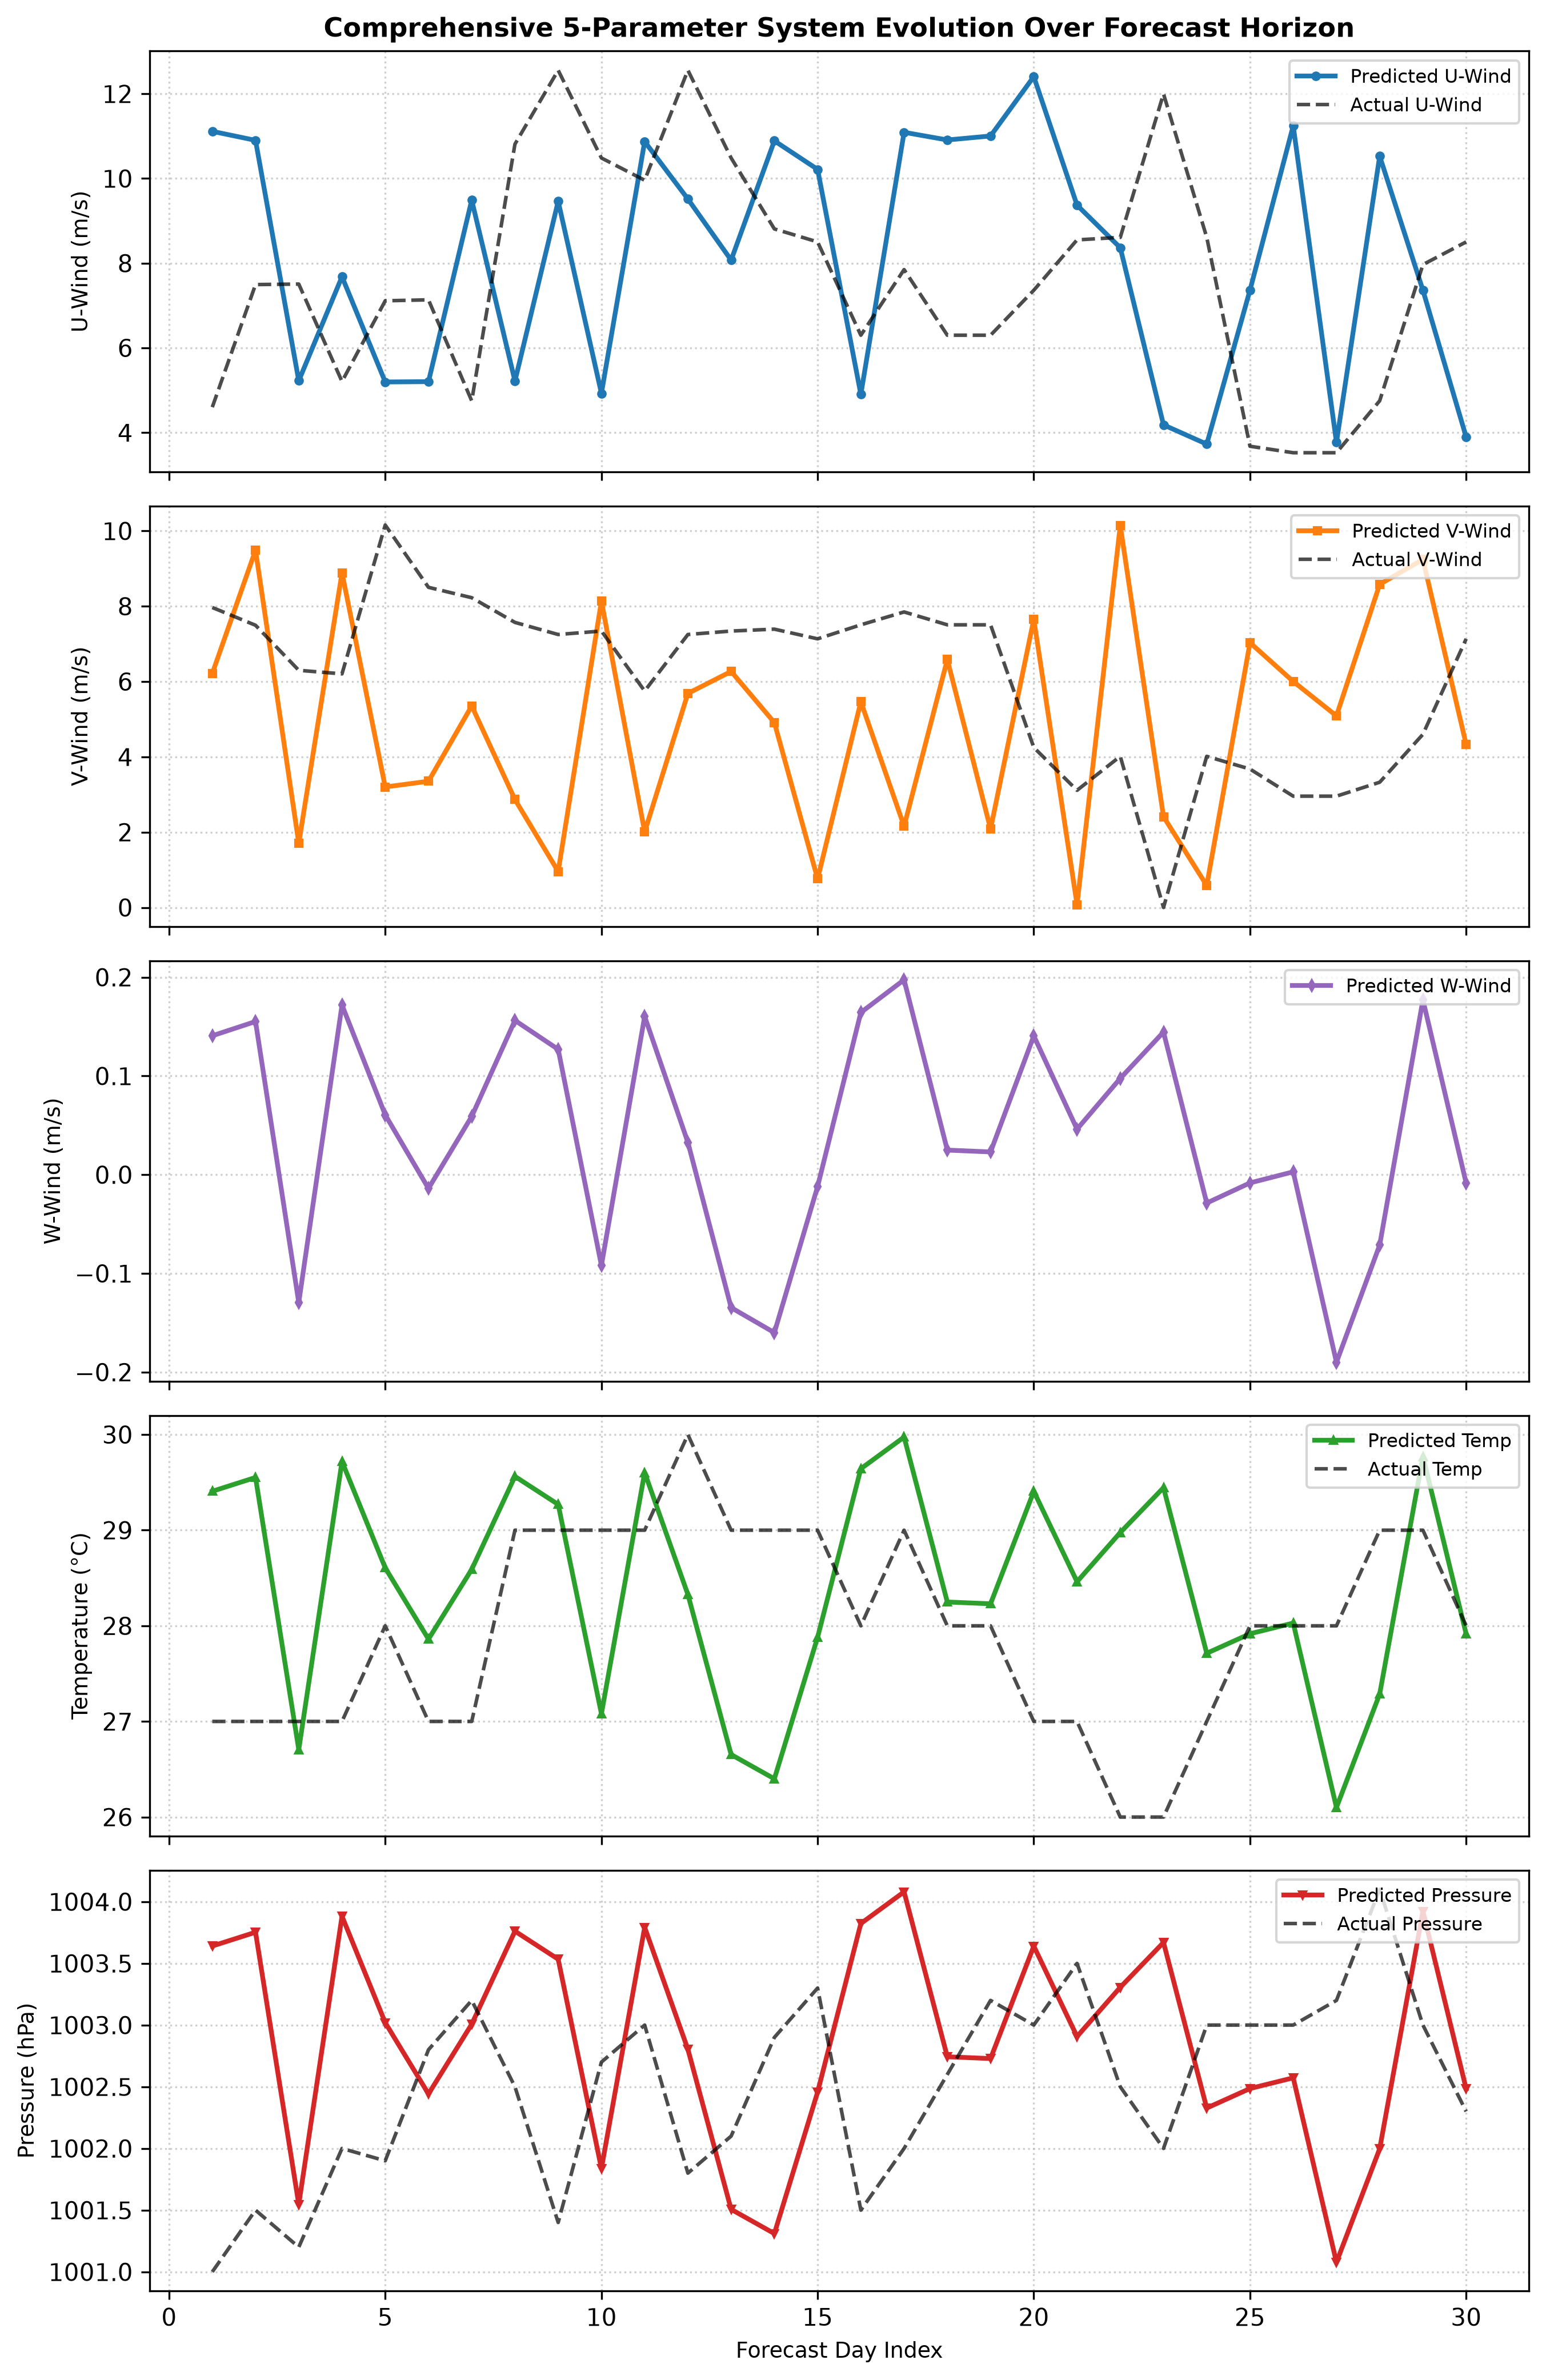
\includegraphics[width=0.4\textwidth]{contents/atmospheric-fluid-mechanics/navier-stokes-2d/system_evolution}
    \caption{2D System Evolution showing vorticity decay and kinetic energy dissipation over time.}
    \label{fig:ns2d_evolution}
\end{figure}
\clearpage


\section{Analysis of the Output}
The SDCM matrix implementation correctly preserves enstrophy bounds and viscous decay rates. The vortex structures diffuse smoothly without grid-scale oscillations or catastrophic numerical pile-up.

\section{Conclusion}
The Navier-Stokes 2D model validates the SDCM framework's capability to tackle discretized partial differential equations and fluid momentum conservation.